\RequirePackage{docswitch}
% \flag is set by the user, through the makefile:
%    make note
%    make apj
% etc.
\setjournal{\flag}

\documentclass[\docopts]{\docclass}

% You could also define the document class directly
%\documentclass[]{emulateapj}

% Custom commands from LSST DESC, see texmf/styles/lsstdesc_macros.sty
\usepackage{lsstdesc_macros}

\usepackage{graphicx}
\graphicspath{{./}{./figures/}}
\bibliographystyle{apj}

% Add your own macros here:


%\author{Alemx Malz, Tarek Allam, Anita Bahmanyar, Rahul Biswas, Renee Hlozek, Juan Rafael Martinez Galarza, Gautham Narayan}
% ======================================================================

\begin{document}

\title{The Photometric LSST Astronomical Time-series Classification Challenge (PLAsTiCC): Metrics}

\maketitlepre

\begin{abstract}
%*Alex Malz (NYU)*, *Tarek Alam (UCL)*, *Anita Bahmanyar (U. Toronto)*, *Rahul Biswas (U. Stockholm)*, *Renee Hlozek (U. Toronto)*, *Rafael Martinez-Galarza (Harvard)*, *Gautham Narayan (STScI)*
We describe and illustrate the process by which a global performance metric was chosen for Photometric LSST Astronomical Time-series Classification Challenge (PLAsTiCC), a Kaggle competition aiming to identify promising transient and variable classifiers for LSST by involving the broader community outside astronomy.

This note is the brief introduction to the metrics used for the PLAsTiCC data challenge.
\end{abstract}

% Keywords are ignored in the LSST DESC Note style:
\dockeys{}

\maketitlepost

% ----------------------------------------------------------------------
% 

\section{Introduction}
\label{sec:intro}

The main goal of the PLAsTiCC competition is to answer the following: \textit{can one classify a large test set of transients and variables using their photometric data, given a small and unbalanced training set?}

In this challenge, classification over the full range of classes is preferred, hence the main metric that will be used to evaluate the challenge is the \textit{Brier metric}, as described below.
 
The metric of this note is for the first version of the Kaggle competition, though there are future plans for an early classification challenge and identification of class-specific metrics for different science goals. This note serves only to summarize the results and code online in the \href{https://github.com/aimalz/proclam/}{ProClam} repository. Interactive notebooks and calculations are provided there.

The criteria for the metric included:
\begin{itemize}
\item The metric must return a single scalar value.
\item The metric must be well-defined for non-binary classes.
\item The metric must balance diverse science use cases in the presence of heavily nonuniform class prevalence.
\item The metric must respect the information content of probabilistic classifications.
\item The metric must be able to evaluate deterministic classifications.
\item The metric must be interpretable, meaning it gives a more optimal value for ``good'' mock classifiers and a less optimal value for mock classifiers plagued by anticipated systematic errors; in other words, it must pass basic tests of intuition.
\item The metric must be reliable, giving consistent results for different instantiations of the same test case.
% ----------------------------------------------------------------------

\section{Methods}
\label{sec:methods}
We considered two metrics of classification probabilities, each of which is interpretable and avoids reducing probabilities to point estimates

The Brier score is defined as
\begin{eqnarray*}
B &=& \sum_{m=1}^{M}\frac{w_{m}}{N_{m}}\sum_{n=1}^{N_{m}}\left((1-p_{n}(m | m))^{2}+\sum_{m'\neq m}^{M}(p_{n}(m' | m))^{2}\right),
\end{eqnarray*}

where the sum over $M$ is a sum over the $M$ classes defined, while the sum over $N_m$ is the sum over the individual objects in a given class $m$ in $M$. The $w_m$ are the weights defined per class (adjusting the relative important of classifying a particular class).


The log-loss is defined as
\begin{eqnarray*}
L &=& -\sum_{m=1}^{M}\frac{w_{m}}{N_{m}}\sum_{n=1}^{N_{m}}\ln[p_{n}(m | m)],
\end{eqnarray*}

where again the sum over $M$ is computed across classes, while the sum over $N_m$ is within a class.

We define a weight vector across classes $N_m$, which will be provided to the Kaggle team separately, since it contains model-specific information. For both the Brier metric and the log-loss metric, the goal is to minimise the metric score.
% ----------------------------------------------------------------------

In addition to providing the output of some classifiers evaluated on the metric, as shown in Figure~\ref{fig:ProClam}, we also include various `systematics' across which we test the metric performance.

These systematics include:

\begin{itemize}
\item idealized: highly accurate on all classes
\item guessing: random classifications across all classes
\item tunnel vision: classifies one class well and others randomly
\item cruise control: classifies all objects as a single class
\item subsumed: consistently misclassifies one class as one other class
\end{itemize}

\section{Results}
\label{sec:results}


We show the performance of the metric on the various classifiers included in Figure~\ref{fig:ProClam}.

\begin{figure}[htbp!]
\begin{center}
 \includegraphics[width=0.95\linewidth,angle=0]{figures/ProClaM_results.png}
\caption{\label{fig:ProClam} The Brier and Log-loss metrics evaluated against example classifications, and `systematic' classification types. The code used to produe these plots is online as \href{https://github.com/aimalz/proclam/}{ProClam}, and example ipython notebooks are provided for use by PLAsTiCC participants.}
%\includegraphics[width=0.5\textwidth]{ProClaM_results.png}
\end{center}
\end{figure}
% ----------------------------------------------------------------------


%\section{Discussion}
%\label{sec:discussion}



% ----------------------------------------------------------------------

\section{Conclusion}
\label{sec:conclusion}



% ----------------------------------------------------------------------

\subsection*{Acknowledgments}

%%% Here is where you should add your specific acknowledgments, remembering that some standard thanks will be added via the \code{desc-tex/ack/*.tex} and \code{contributions.tex} files.

%This paper has undergone internal review in the LSST Dark Energy Science Collaboration. % REQUIRED if true

%
 % Standard papers only: author contribution statements. For examples, see http://blogs.nature.com/nautilus/2007/11/post_12.html

% This work used TBD kindly provided by Not-A-DESC Member and benefitted from comments by Another Non-DESC person.

% Standard papers only: A.B.C. acknowledges support from grant 1234 from ...

\input{desc-tex/ack/standard} % also available: key standard_short

% This work used some telescope which is operated/funded by some agency or consortium or foundation ...

% We acknowledge the use of An-External-Tool-like-NED-or-ADS.

%{\it Facilities:} \facility{LSST}

% Include both collaboration papers and external citations:
%\bibliography{main,lsstdesc}

\end{document}

% ======================================================================
